
%
%
%
\section*{AIM:}
To light up LEDs in a ring counter pattern using the parallel port
\section*{THEORY:}
A parallel port is a type of interface found on computers (personal and otherwise) for connecting peripherals. In computing, a parallel port is a parallel communication physical interface. It is also known as a printer port or Centronics port. The port is composed of 4 control lines, 5 status lines and 8 data lines. The connector for the parallel port is a 25 pin D-Type female connector. The parallel port pinout is as shown below:

\begin{figure}[h]
\centering
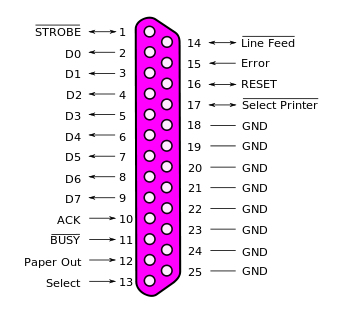
\includegraphics[scale=0.5]{pp}
\caption{Parallel port pinout}
\end{figure}

The parallel port has three commonly used port addresses as shown below:

\newpage
\begin{table}[h]
\centering
\bgroup
\def\arraystretch{1.5}
\begin{tabular}{ |c|p{7cm}| }
\hline
\textbf{Address} & \textbf{Notes}\\
\hline
3BCh - 3BFh & Used for parallel ports which were incorporated onto Video cards - doesn't support ECP addresses\\
\hline
378h - 37Fh & Usual address for LPT1\\
\hline
278h - 27Fh & Usual address for LPT2\\
\hline
\end{tabular}
\caption{Parallel port base addresses}
\egroup
\end{table}

The parallel port is associated with three software registers namely- the data port, the status port, and the control port.
These ports can be used to read/write data and control the operation of the parallel port. A detailed description of the individual bits in these registers is given below:

\begin{table}[h]
\centering
\bgroup
\def\arraystretch{1.5}
\begin{tabular}{|c|c|c|c|c|}
\hline
\textbf{Offset}           & \textbf{Name}              & \textbf{Read/Write}    & \textbf{Bit No.} & \textbf{Properties} \\ \hline
\multirow{8}{*}{Base + 0} & \multirow{8}{*}{Data Port} & \multirow{8}{*}{Write} & Bit 7            & Data 7              \\ \cline{4-5} 
                          &                            &                        & Bit 6            & Data 6              \\ \cline{4-5} 
                          &                            &                        & Bit 5            & Data 5              \\ \cline{4-5} 
                          &                            &                        & Bit 4            & Data 4              \\ \cline{4-5} 
                          &                            &                        & Bit 3            & Data 3              \\ \cline{4-5} 
                          &                            &                        & Bit 2            & Data 2              \\ \cline{4-5} 
                          &                            &                        & Bit 1            & Data 1              \\ \cline{4-5} 
                          &                            &                        & Bit 0            & Data 0              \\ \hline
\end{tabular}
\caption{Data Port register bits}
\egroup
\end{table}

The data port is simply used for outputting data on the Parallel Port's data lines (Pins 2-9). This register is normally a write only port. However, modern parallel ports are often bi-directional, and data can be read from the data port address.

\begin{table}[h]
\centering
\bgroup
\def\arraystretch{1.5}
\begin{tabular}{|c|c|c|c|c|}
\hline
\textbf{Offset}           & \textbf{Name}                & \textbf{Read/Write}        & \textbf{Bit No.} & \textbf{Properties} \\ \hline
\multirow{8}{*}{Base + 1} & \multirow{8}{*}{Status Port} & \multirow{8}{*}{Read Only} & Bit 7            & Busy                \\ \cline{4-5} 
                          &                              &                            & Bit 6            & Ack                 \\ \cline{4-5} 
                          &                              &                            & Bit 5            & Paper Out           \\ \cline{4-5} 
                          &                              &                            & Bit 4            & Select In           \\ \cline{4-5} 
                          &                              &                            & Bit 3            & Error               \\ \cline{4-5} 
                          &                              &                            & Bit 2            & IRQ                 \\ \cline{4-5} 
                          &                              &                            & Bit 1            & Reserved            \\ \cline{4-5} 
                          &                              &                            & Bit 0            & Reserved              \\ \hline
\end{tabular}
\caption{Status Port register bits}
\egroup
\end{table}

The Status Port is a read only port. Any data written to this port will be ignored. The Status Port is made up of 5 input lines (Pins 10,11,12,13 \& 15), an IRQ status register and two reserved bits.
\newpage
\begin{table}[]
\centering
\bgroup
\def\arraystretch{1.5}
\begin{tabular}{|c|c|c|c|c|}
\hline
\textbf{Offset}           & \textbf{Name}                 & \textbf{Read/Write}         & \textbf{Bit No.} & \textbf{Properties}        \\ \hline
\multirow{8}{*}{Base + 2} & \multirow{8}{*}{Control Port} & \multirow{8}{*}{Read/Write} & Bit 7            & Unused                     \\ \cline{4-5} 
                          &                               &                             & Bit 6            & Unused                     \\ \cline{4-5} 
                          &                               &                             & Bit 5            & Enable Bi-Directional Port \\ \cline{4-5} 
                          &                               &                             & Bit 4            & Enable IRQ via ACK line    \\ \cline{4-5} 
                          &                               &                             & Bit 3            & Select Printer             \\ \cline{4-5} 
                          &                               &                             & Bit 2            & Initialize Printer (Reset) \\ \cline{4-5} 
                          &                               &                             & Bit 1            & Auto Linefeed              \\ \cline{4-5} 
                          &                               &                             & Bit 0            & Strobe                     \\ \hline
\end{tabular}
\caption{Control Port register bits}
\egroup
\end{table}

The Control Port (base address + 2) was intended as a write only port. When a printer is attached to the Parallel Port, four "controls" are used. These are Strobe, Auto Linefeed, Initialize and Select Printer, all of which are inverted
except Initialize.

The printer would not send a signal to initialize the computer, nor would it tell the computer to use auto linefeed. However these four outputs can also be used for inputs. If the computer has placed a pin high (e.g. +5v) and your device wanted to take it low, you would effectively short out the port, causing a conflict on that pin. Therefore these lines are "open collector" outputs (or open drain for CMOS devices). This means that it has two states. A low state (0v) and a high impedance state (open circuit).

Bits 4 \& 5 are internal controls. Bit four will enable the IRQ (See Using the Parallel Ports IRQ) and Bit 5 will enable the bi-directional port meaning so as to enable input of 8 bits using (DATA0-7). This mode is only possible if the card supports it. Bits 6 \& 7 are reserved. Any writes to these two bits will be ignored. 

\section*{PROCEDURE:}
\textbf{\underline{STEP 1}:} 
Setup a circuit connecting the parallel port to 4 LEDs.

\textbf{\underline{STEP 2}:} Compile and run the program given below in Linux environment with super user privilege.

The four LEDs will be seen lighting up in the ring counter pattern.

\section*{PROGRAM:}
\begin{lstlisting}
#include <stdio.h>
#include <sys/io.h>
#include <unistd.h>

void main(){

     int base = 0x378;
     if( ioperm(base, 1, 1) == -1){
          printf("\nError granting permission.Terminating...\n");
          return;
     }else{}
     
     int i;
     //--outputting powers of 2 from 1 to 16, one in every second
     
     for(i=1 ; ; i=1)
          for(; i<16 ; sleep(1), i = i<<1)
               outb(i);
     
     ioperm(base, 1, 0);
     return;  
}
\end{lstlisting}

\section*{RESULT:}
The program has been executed and the output, verified.
%
%

